% This is samplepaper.tex, a sample chapter demonstrating the
% LLNCS macro package for Springer Computer Science proceedings;
% Version 2.21 of 2022/01/12
%
\documentclass[runningheads, 10pt]{llncs}
%
\usepackage[T1]{fontenc}
% T1 fonts will be used to generate the final print and online PDFs,
% so please use T1 fonts in your manuscript whenever possible.
% Other font encondings may result in incorrect characters.
%
\usepackage{subcaption}
\usepackage{graphicx}
\usepackage{amsmath}
\usepackage{booktabs}
\usepackage{tabularx}
\usepackage{float}
\usepackage{listings}
\usepackage{multicol}
\setlength{\heavyrulewidth}{1.5pt}
\setlength{\abovetopsep}{4pt}
\lstdefinestyle{custompython}{
	language=Python,
	basicstyle=\ttfamily\footnotesize,
	keywordstyle=\color{blue},
	commentstyle=\color{green},
	stringstyle=\color{magenta},
	showstringspaces=false,
	breaklines=true,
	breakatwhitespace=false,
	columns=fullflexible,
	keepspaces=true,
	frame=single,
	tabsize=4
}
% Used for displaying a sample figure. If possible, figure files should
% be included in EPS format.
%
% If you use the hyperref package, please uncomment the following two lines
% to display URLs in blue roman font according to Springer's eBook style:
% \urlstyle{rm}
%
\usepackage[english]{babel}
\usepackage{csquotes}
\usepackage{hyperref}
\usepackage[style=lncs, backend=biber, natbib=true]{biblatex}
\usepackage{lipsum}
\usepackage{color}
\renewcommand\UrlFont{\color{blue}\rmfamily}

\addbibresource{wr227.bib}

\begin{document}
%
\title{Can LLMs Generalize to Structured Classification Tasks? A Comparative Analysis with Traditional Machine Learning Models in an Educational Context}
%
\titlerunning{Can LLMs Generalize to Structured Classification Tasks?}
% If the paper title is too long for the running head, you can set
% an abbreviated paper title here
%
\author{Thien-Lac Quach\inst{1,2}\orcidID{0009-0004-6310-5149}\and
Ton-Minh-Ky Tran\inst{1,2}\orcidID{0009-0006-5027-2516}}
%
\authorrunning{Quach \& Tran} 
% First names are abbreviated in the running head.
% If there are more than two authors, 'et al.' is used.
%
\institute{Faculty of Information Technology, University of Science, Ho Chi Minh City, Vietnam \and
Vietnam National University, Ho Chi Minh City, Vietnam
\email{\{24125092,24125102\}@apcs.fitus.edu.vn}}
%
\maketitle              % typeset the header of the contribution
%
\begin{abstract}
While Large Language Models (LLMs) excel in natural language processing, their ability to generalize to structured, non-linguistic tasks remains uncertain. This paper investigates this gap by comparing general-purpose LLMs and traditional machine learning models in a specific educational context--predicting students' final academic outcomes--using the Open University Learning Analytics Dataset (OULAD). To assess baseline generalization without task-specific adaptation, we deliberately exclude fine-tuning and retrieval-augmented generation. Instead, we evaluate two open-weight, small-size LLMs, Qwen-2.5-3B and LLaMA-3-8B, interpreting serialized JSON tabular data using zero-shot, one-shot, and five-shot prompting. These are benchmarked against seven hyperparameter-tuned traditional models, including Random Forest and Gradient Boosting. Our results demonstrate a severe performance gap: traditional ensemble methods significantly outperformed the LLMs, with the best-performing LLM peforming no better than chance. These findings highlight that current general-purpose LLMs struggle to interpret numerical feature vectors, making them currently unsuitable for complex and tabularized data compared to traditional classifiers. Future research should explore domain adaptation techniques or architectural modifications to bridge this modality gap. 
\keywords{Large Language Models \and Traditional Machine Learning Models \and Classification problem \and Generalization \and Education}
\end{abstract}
%
%
\newpage

\begin{multicols}{2}
\sloppy
\raggedright
\section{Introduction}
Large Language Models (LLMs) have seen an unprecedented rise in popularity and application across various domains, including education. This integration of LLMs into education contexts has generated considerable interest, driven by their demonstrated proficiency in natural language understanding, text generation, and reasoning tasks \cite{Brown2020}. However, while LLMs excel in natural language processing, one must pose the question: how well can these models generalize beyond language generation to perform effectively in structured, non-linguistic tasks, such as tabular classification? This question carries practical significance for Higher Education Institutions (HEIs), where the ability to predict students' academic outcomes from behavioral and demographic data underpins early-warning systems that identify at-risk students and allocate support resources.

Regarding classification tasks, there exists an extensive, well-established literature on the use of traditional machine learning models, such as Random Forest, Gradient Boosting, and Support Vector Machines, to address such problems. These models are explicitly trained on the target dataset, benefit from hyperparameter tuning, and operate natively on tabular feature vectors. Their effectiveness is well-documented \cite{Delgado2014, Jimenez-Macias2025, Zhan2025, Bujang2021, Alhakbani2022}. LLMs, by contrast, acquire knowledge through large-scale pretraining on textual corpora and are not exposed to structured tabular data during this process. For instance, when presented with a student record serialized as JSON, the LLM must interpret a data format fundamentally different from the natural language it was trained on.

Recent studies have begun examining LLM performance on tabular data. Wen et al. (2025) proposed Tabular In-Context Learning (TabICL), a retrieval-augmented framework that adapts LLMs for tabular classification \cite{Wen2025}. However, such approaches incorporate task-specific mechanisms (retrieval pipelines, structured prompting protocols) that blur the line between general-purpose inference and task-adapted learning. Furthermore, most existing comparisons operate on generic benchmarks (e.g., UCI, OpenML datasets) rather than domain-specific datasets with complex, multi-source feature engineering pipelines, a common characteristic of real-world educational data.

This gap motivates our central research question: To what extent can general-purpose LLMs, without any task-specific adaptation, generalize to a structured classification task, particularly in an educational context? We therefore deliberately exclude fine-tuning techniques (e.g., LoRA, QLoRA) and retrieval-augmented generation (RAG), as these modifications would transform the LLM into a task-adapted model, answering a different research question — namely, how much domain-specific adaptation is required to close the performance gap. To this end, we also favor simple prompting strategies (zero-shot, one-shot, few-shot) that do not require engineering complex prompt templates or retrieval mechanisms, as these would again shift the focus from generalization to adaptation.

To this end, we evaluate two open-weight LLMs, Qwen-2.5-3B and LLaMA-3-8B, using zero-shot, one-shot, and five-shot prompting on the Open University Learning Analytics Dataset (OULAD) \cite{Kuzilek2017} and benchmark these against seven traditional machine learning models that undergo full hyperparameter tuning via cross-validation. We also designed a pipeline to serialize tabular data into a JSON format that is compatible with LLM input, ensuring that the evaluation reflects the LLMs' ability to interpret structured data rather than relying on engineered prompt templates. Our findings reveal that the tested LLMs underperform heavily compared to traditional models, with the best LLM configuration achieving a Macro F1 of 0.481, while the best traditional model reaches 0.722. This significant performance gap highlights the limitations of general-purpose LLMs in structured classification tasks and underscores the need for further research into domain adaptation techniques or architectural modifications to enhance their applicability in non-linguistic contexts.

The remainder of this paper is organized as follows. Section 2 provides background on the models used. Section 3 reviews related work on machine learning classifiers in education, data aggregation, and performance metrics. Section 4 describes the methodology, including the dataset, preprocessing pipeline, and experimental setup. Section 5 presents the results, and Section 6 discusses their implications, limitations, and directions for future work.
\section{Background}
\subsection{Traditional Machine Learning Models}

This paper uses seven traditional machine learning models for the classification task: Random Forest, Support Vector Machine, Gradient Boosting, Decision Tree, $k$-Nearest Neighbors, Extreme Learning Machine (ELM), and Multilayer Perceptron (MLP). The rationale for selecting these models is explained in the Methodology section. Below is a brief introduction to each model.

\subsubsection{Random Forest}

Random Forest (RF) is an ensemble learning method first proposed by Ho in 1995 \cite{Ho1995} and later developed by Breiman and Cutler \cite{Breiman2001}. The algorithm grows multiple decision trees and combines their outputs to produce a final prediction. Each tree is trained using a random vector $\Theta$, generated independently from past vectors but with the same distribution \cite{Breiman2001}. The final prediction is obtained by aggregating ("voting") the predictions of all trees, typically via majority vote for classification \cite{Breiman2001}. RF is known for its robustness to overfitting, ability to handle high-dimensional data, and effectiveness in capturing complex interactions between features \cite{Breiman2001}. It remains one of the most effective machine learning models despite its early introduction \cite{Delgado2014}.

\subsubsection{Support Vector Machine}

Support Vector Machine (SVM) is a supervised learning model based on a simple idea: find an optimal hyperplane that separates the input data into different classes. The optimal hyperplane is defined as the one that maximizes the margin between classes, where the margin is the distance between the hyperplane and the nearest training points from each class (support vectors) \cite{Cortes1995}. SVM can be extended to handle non-linearly separable data by using kernel functions, particularly the Gaussian Radial Basis Function (RBF) kernel, which maps inputs into a higher-dimensional feature space where a linear separation is possible \cite{Schoelkopf2002}. SVM is widely used for classification tasks due to its effectiveness in high-dimensional spaces and its ability to model complex relationships between features and classes \cite{Hsu2003}.

\subsubsection{Gradient Boosting}

Gradient Boosting (GB) is an ensemble learning method that builds a series of weak learners, typically trees, that learn from the residuals of previous learners. Residuals are the differences between the predicted values and the actual values of the target variable \cite{Chen2024}. The training algorithm iterates through $M$ boosting rounds. In each round $m$, a new weak learner $T_{(m)}$ is trained to predict the residuals, thereby rectifying mistakes made by previous learners \cite{Chen2024}. The final prediction is obtained by summing the predictions of all weak learners, weighted by a learning rate $\nu$ that controls each learner's contribution \cite{Friedman2001}. The prediction process works as follows: for each tree $T_{(m)}$ and test instance $x_i$, the output $T_m(x_i)$ is scaled by $\nu$ and added to the cumulative prediction from previous trees, resulting in
\[
	F_M(x_i) = \sum_{m=1}^M \nu T_m(x_i). 
\]
GB is known for its high predictive accuracy and is widely used in various applications, including classification and regression tasks \cite{Friedman2001}.

\subsubsection{Decision Tree}

Decision Tree (DT) is a supervised learning model that recursively partitions the feature space into regions that are as homogeneous as possible with respect to the target label. At each internal node, the algorithm selects a feature (and a threshold for numerical features) that maximizes an impurity reduction criterion such as Gini impurity or information gain. Predictions are obtained by following the decision rules from the root to a leaf and outputting the majority class for classification tasks. Decision trees are interpretable and can capture non-linear decision boundaries, but they may overfit without appropriate regularization (e.g., maximum depth, minimum samples per split/leaf, or pruning).

\subsubsection{$k$-Nearest Neighbors}

$k$-Nearest Neighbors ($k$-NN) is a non-parametric, instance-based learning algorithm that classifies a data point based on the majority class among its $k$ nearest neighbors in feature space \cite{Cover1967}. Distance between data points is typically measured by Euclidean distance, although other measures such as Pearson or Spearman distance can also be used \cite{Jaskowiak2011}. The choice of the algorithm's sole hyperparameter, $k$, is crucial for performance. A larger value of $k$ can make the model more robust to noise, though it may blur interclass boundaries \cite{Everitt2011}. Due to its simplicity, $k$-NN's accuracy can be significantly affected by the choice of $k$ and the nature of the data, and it often requires feature scaling to ensure that all features contribute equally to the distance calculations \cite{Nigsch2006}. $k$-NN is noted for its strong consistency: as the dataset size increases, the probability of $k$-NN making an error converges to no worse than twice the Bayes error rate, which is the lowest possible error rate for any classifier \cite{Cover1967}.

\subsubsection{Extreme Learning Machine}

Extreme Learning Machine (ELM) is a type of feedforward neural network, first proposed by Huang et al. in 2006 \cite{Huang2006}. ELM is a learning algorithm for single-hidden layer feedforward neural networks (SLFNs) whose training is significantly faster than traditional counterparts. ELM randomly assigns input weights and hidden-layer biases, and then analytically determines the output weights by solving a linear system of equations \cite{Huang2006}. The training process consists of three steps: (1) randomly generate the input weights and hidden-layer biases; (2) compute the hidden-layer output matrix; (3) calculate the output weights using the Moore--Penrose generalized inverse of the hidden-layer output matrix \cite{Huang2006}. ELM has been shown to achieve good generalization performance with significantly reduced training time compared to traditional feedforward neural networks, making it suitable for large-scale classification tasks \cite{Huang2012}.

\subsubsection{Multilayer Perceptron}

Multilayer Perceptron (MLP) is a class of feedforward artificial neural network that consists of at least three layers: an input layer, one or more hidden layers, and an output layer \cite{Rosenblatt1958}. First proposed by Rosenblatt in 1958, MLP also serves as a basis for more complex neural network architectures, upon which ELM is built. Crucial in MLP architecture are the concepts of units and hidden layers. Units, also known as neurons, are the basic computational elements of MLP that receive input, process it, and produce output. Hidden layers are the layers of units that exist between the input and output layers, allowing MLP to learn complex representations of data \cite{Rosenblatt1958}. MLP functions by assigning weights to the connections between units and applying an activation function (commonly a sigmoid or ReLU function) to the output of each neuron. Learning in MLP is typically achieved through backpropagation and gradient descent algorithms, which adjust the weights to minimize the error between the predicted and actual outputs (modeled by a loss function) \cite{Haykin1999}.

\subsection{Large Language Models}

Large Language Models (LLMs) present a significant advancement in artificial intelligence, particularly in the field of natural language processing (NLP). The architecture of LLMs is based on the Transformer model, first introduced in a foundational paper by Vaswani et al. in 2017 \cite{Vaswani2017}. The Transformer architecture utilizes self-attention mechanisms to process input data, allowing it to capture long-range dependencies and contextual information effectively \cite{Vaswani2017}. LLMs are trained on enormous amounts of data and often possess billions of parameters, enabling them to generate human-like text and perform a wide range of language tasks with high accuracy \cite{Brown2020}. The training process of LLMs typically involves two stages: pre-training and fine-tuning. During pre-training, the model learns general language patterns from a large corpus of text, while fine-tuning involves further training the model on specific tasks or domains to enhance its performance in those areas \cite{Devlin2018}. LLMs have revolutionized the field in that they can generalize across a wide range of tasks without task-specific training, and they have been shown to outperform traditional machine learning models in various NLP tasks \cite{Brown2020}.

For our paper, we choose two models: \textbf{Qwen-2.5-3B} and \textbf{LLaMA-3-8B} (the suffix $X\text{B}$ of each model's name refers to the number of billions of parameters $X$). These models are publicly available on Hugging Face. Below is a brief introduction to each model.

\subsubsection{Qwen-2.5-3B}

Qwen-2.5-3B is a large language model developed by Alibaba, which is part of the Qwen series of models. The Qwen 2.5 series is designed to be more efficient than its predecessors, especially on coding and mathematical tasks. It has also been reported to enhance 
instruction-following, producing longer responses (beyond 8K tokens), interpreting structured inputs (e.g., tables), and generating structured outputs, particularly in JSON format. It is also more robust to variations in system prompts, which improves role-playing behavior and condition control in chatbot applications.

\subsubsection{LLaMA-3-8B}

LLaMA-3-8B is a large language model developed by Meta as part of the LLaMA series. It is designed to be efficient and capable across diverse language tasks. Architecturally, LLaMA 3 is an autoregressive language model built on an optimized Transformer backbone. Its tuned variants are aligned with human preferences for helpfulness and safety through supervised fine-tuning (SFT), followed by reinforcement learning from human feedback (RLHF).
\section{Related Work}
\subsection{Machine Learning Models as Classifiers in Educational Context}
The use of machine learning models as classifiers in educational contexts has been explored in various studies \cite{Jimenez-Macias2025, Zhan2025, Tong2025, Alhakbani2022}. From these studies, two main conclusions can be drawn.

First, certain models often outperform others in terms of accuracy for general classification tasks. Most prominently, ensemble methods---particularly Random Forest (RF)---consistently rank as top performers: Delgado et al. (2014) established RF as a "gold standard" across 179 classifiers \cite{Delgado2014}, a finding echoed in educational contexts by Jimenez-Macias et al. (2025) \cite{Jimenez-Macias2025}. Support Vector Machines and Artificial Neural Networks also prove effective for capturing non-linear relationships in educational data, with reported accuracies reaching 97.88\% and 99\%, respectively \cite{Zhan2025, Alhakbani2022}. Gradient Boosting variants such as XGBoost have also shown similar strength in identifying at-risk students \cite{Alhakbani2022, Delgado2014}. More recently, stacking ensemble models have been explored; these methods train heterogeneous base learners (e.g., KNN, Naive Bayes, RF, and XGBoost) and aggregate their outputs using a meta-learner such as Logistic Regression to mitigate individual model biases. For instance, a stacking framework achieved an accuracy of 98.53\% in predicting learning achievements on the XuetangX MOOC dataset \cite{Tong2025}.

Second, a critical consensus across current literature is the superiority of behavioral engagement data over demographic information for classification tasks. Online behavioral logs, including video watch counts, forum posts, and quiz participation, are significantly more influential in predicting academic risk than static factors like age, gender, or educational background. Jimenez-Macias et al. (2025) further refined this by demonstrating that time spent on tasks is a more sensitive predictor of performance than the raw number of attempts \cite{Jimenez-Macias2025}. Moreover, the distribution of grades across interactions significantly impacts model accuracy, as uniform grade distributions enhance the algorithm's ability to generalize patterns and make accurate predictions \cite{Jimenez-Macias2025}.

Methodological integrity in this context requires addressing class imbalance and interpretability. Educational datasets are frequently imbalanced, often containing significantly fewer failing students than passing ones \cite{Bujang2021, Tong2025}. To address this, researchers employed data-level solutions like SMOTE (Synthetic Minority Oversampling Technique) or Sequential Conditional GANs to balance class distributions and prevent model bias toward the majority class \cite{Bujang2021}. Furthermore, as models grow in complexity, tools like SHAP (SHapley Additive exPlanations) are increasingly used to provide "white-box" transparency, identifying which specific student behaviors drive the final prediction \cite{Tong2025}.

Despite these advancements, inconsistent preprocessing and feature scaling remain primary challenges, as they are often cited as the reason for varied performance reports for identical models across different studies \cite{Alhakbani2022}. Finally, the emerging paradigm of Tabular In-Context Learning (TabICL) using Large Language Models (LLMs) offers a novel interface for classification that can complement traditional frameworks like XGBoost and CatBoost, which have served as state-of-the-art benchmarks for tabular data for decades \cite{Wen2025}.

\subsection{Data aggregation}
It stands to reason that gathering high-quality and representative data is often a difficult endeavor \cite{Alias2024}. Alias et al. (2024) delineated a framework in which a list of hypothetically relevant features is enumerated and filtered via information gain. More specifically, the features taken into consideration include those relating to students' study hours, participation in extracurricular activities, hours of sleep, and mock exams practiced \cite{Suleiman2024}. Surveys for these features are deployed online as a questionnaire using the platform Google Forms.


\subsection{Performance metrics}
Common metrics to assess classification algorithms include accuracy, precision, recall, F1-score \cite{Alias2024, Zaky2023}, and the area under the receiver operating characteristic curve (AUC-ROC) \cite{Brzezinski2017, Yang2017}. These metrics provide insights into a model's ability to correctly classify instances, handle imbalanced datasets, and make informed decisions based on predictions \cite{Brzezinski2017}. Techniques for handling imbalanced datasets are crucial when working with decision tree (DT)-based models to avoid bias toward the majority class. Here, we focus on the Synthetic Minority Over-sampling Technique (SMOTE), specifically its variant ADASYN, which utilizes a weighted distribution to determine the learning difficulty of minority-class samples and generates synthetic data accordingly \cite{Chawla2011, Elreedy2019}. This approach helps to balance the dataset and improve the performance of decision tree models in predicting the minority class.

\input{Methodology.tex}
\section{Results}

\end{multicols}
	
\begin{table}[H]
\centering
\label{tab:results-summary}
\begin{tabular}{llcc}
\toprule
Model & Technique & Macro F1 & Balanced Acc. \\
\midrule
\multicolumn{4}{l}{\textbf{Traditional ML}} \\
Decision Tree & -- & 0.675 & 0.685 \\
Random Forest & -- & 0.720 & 0.719 \\
Gradient Boosting & -- & 0.722 & 0.718 \\
Support Vector Machine & -- & 0.652 & 0.635 \\
K-Nearest Neighbors & -- & 0.601 & 0.595 \\
MLP Classifier & -- & 0.678 & 0.676 \\
ELM Classifier & -- & 0.645 & 0.630 \\
\addlinespace
\multicolumn{4}{l}{\textbf{LLMs}} \\
Qwen2.5-3B & 0-shot & 0.218 & 0.297 \\
Qwen2.5-3B & 1-shot & 0.387 & 0.562 \\
Qwen2.5-3B & 5-shot & 0.306 & 0.377 \\
Meta-Llama3-9B & 0-shot & 0.280 & 0.341 \\
Meta-Llama3-9B & 1-shot & 0.392 & 0.509 \\
Meta-Llama3-9B & 5-shot & 0.481 & 0.494 \\
\bottomrule
\end{tabular}
\caption{Summary of traditional ML and LLM performance on the test set (Macro F1 and Balanced Accuracy).}
\end{table}
	
\begin{figure}[H]
\centering
	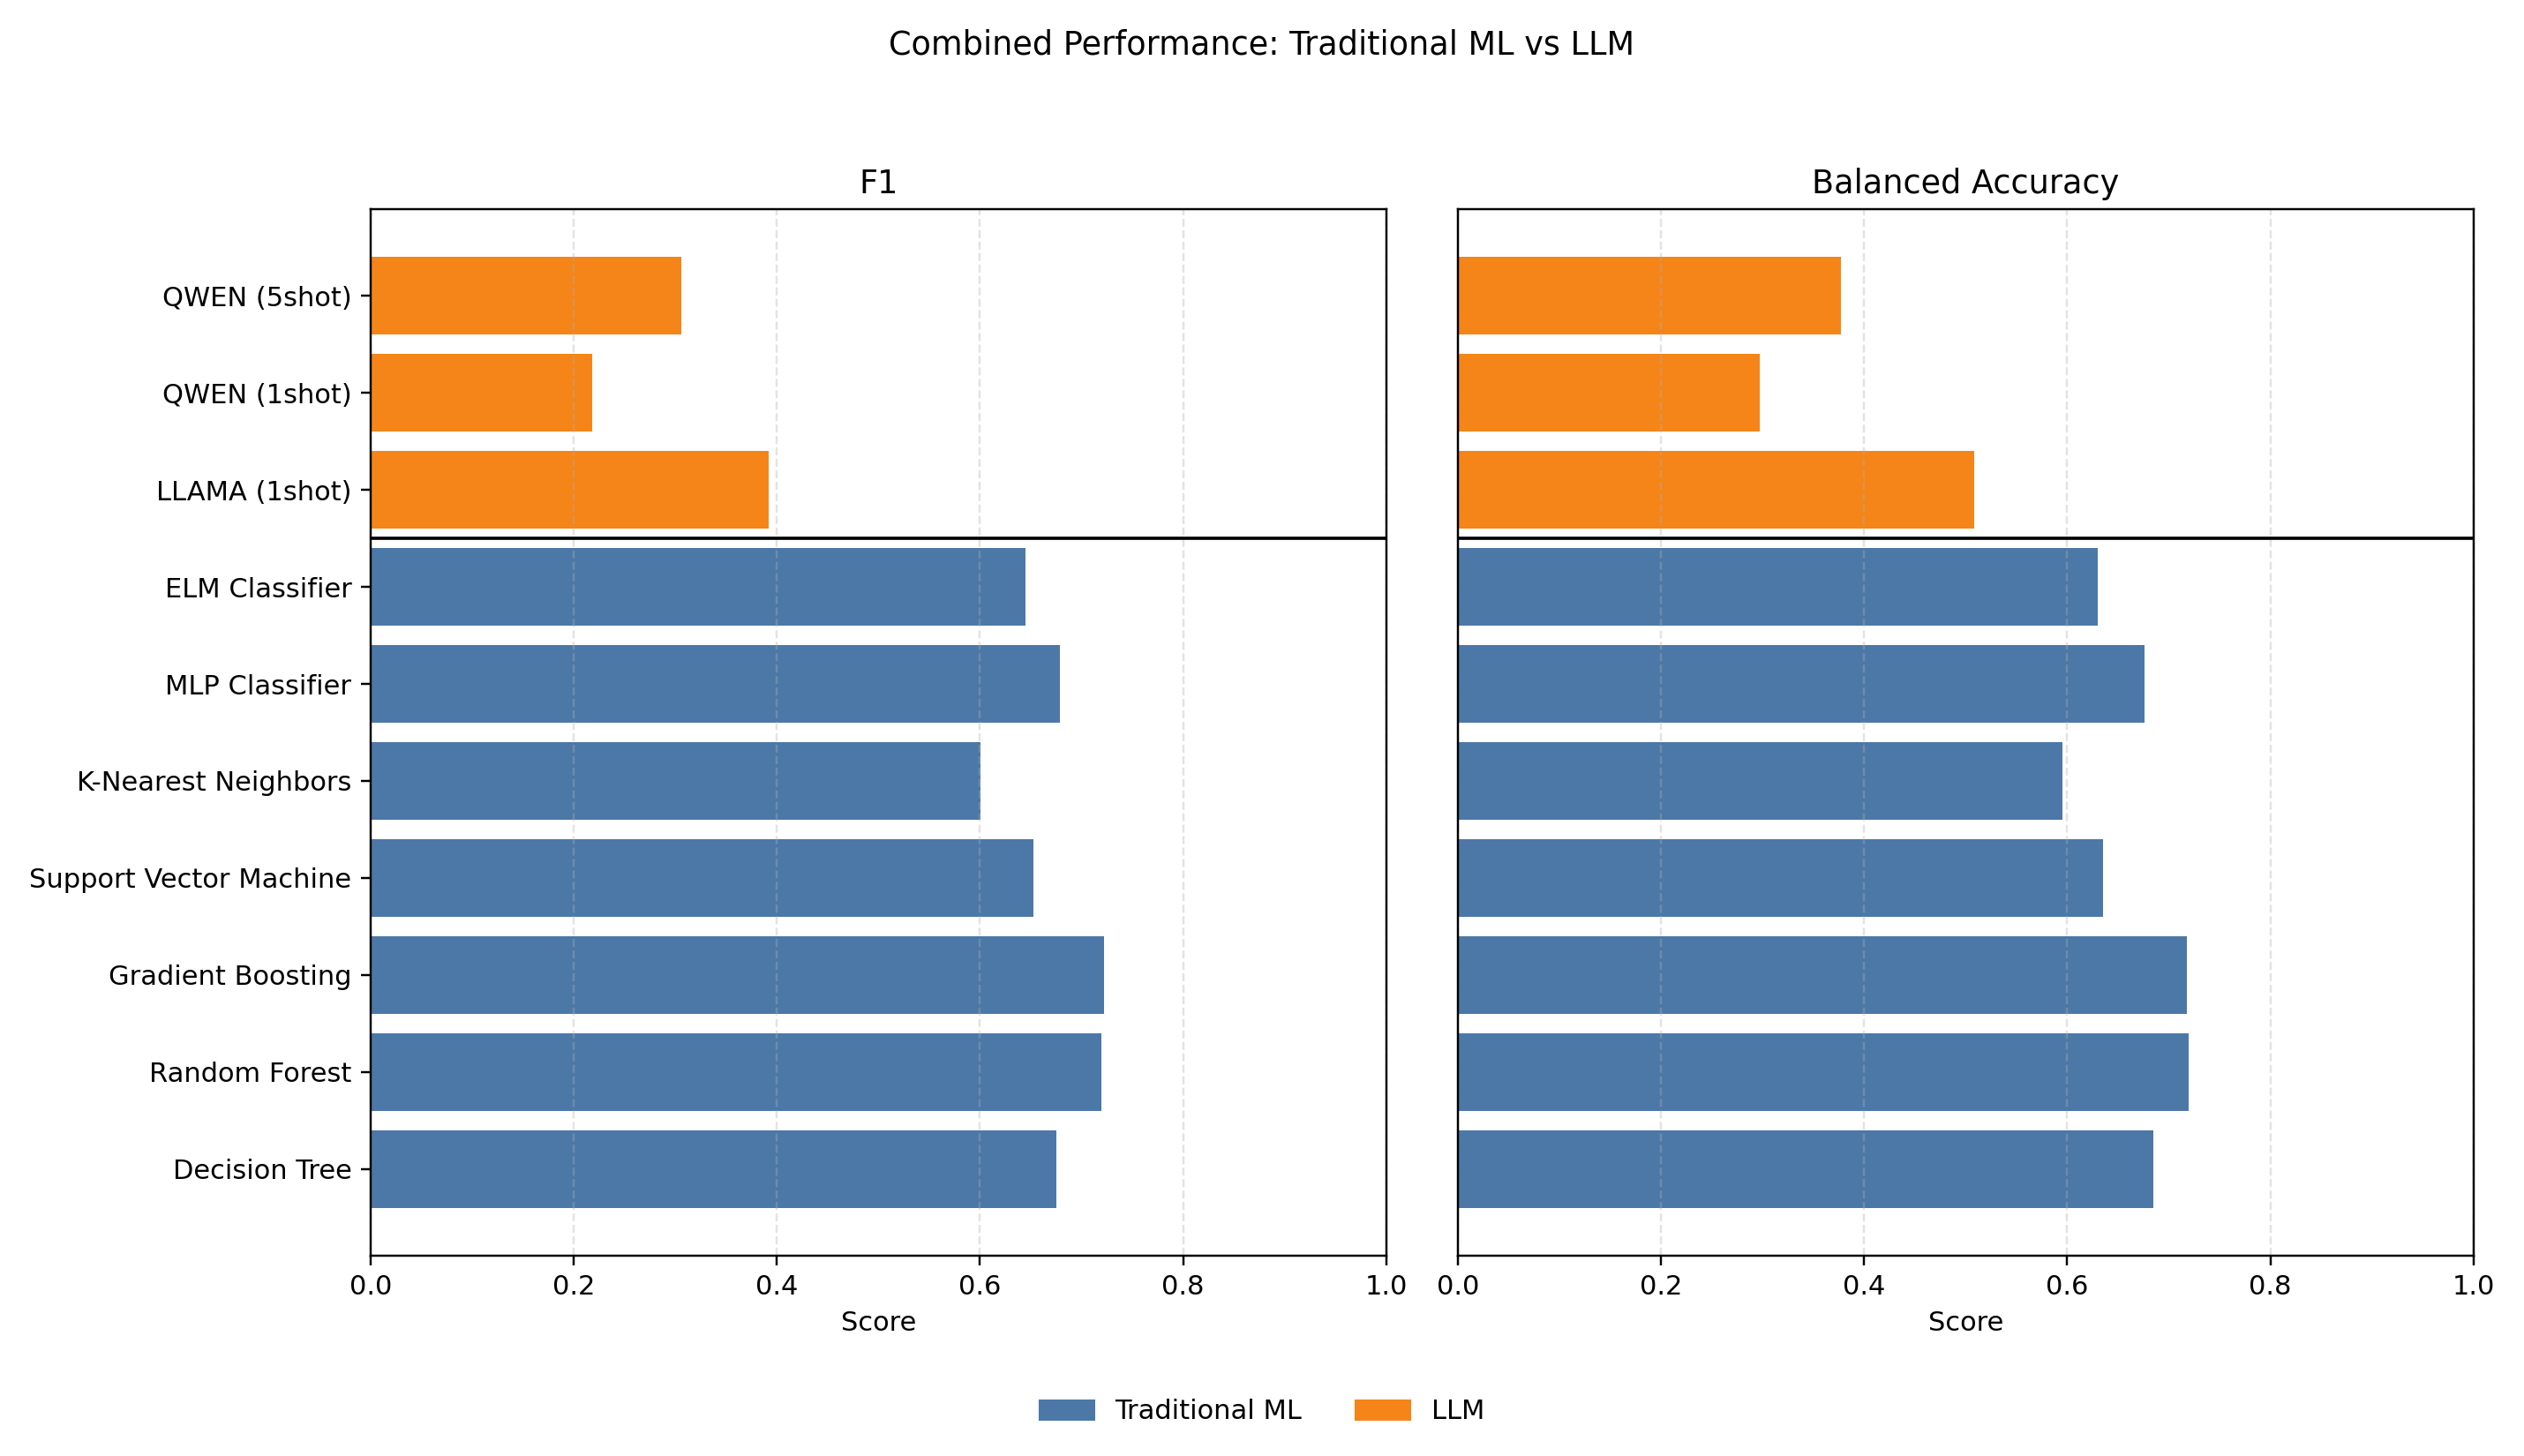
\includegraphics[width=\textwidth]{code/plots/combined_tradml_llm_performance.png}
	\caption{Combined performance comparison of traditional machine learning models and large language models using F1 and Balanced Accuracy.}
\end{figure}

\begin{figure}[H]
\centering
	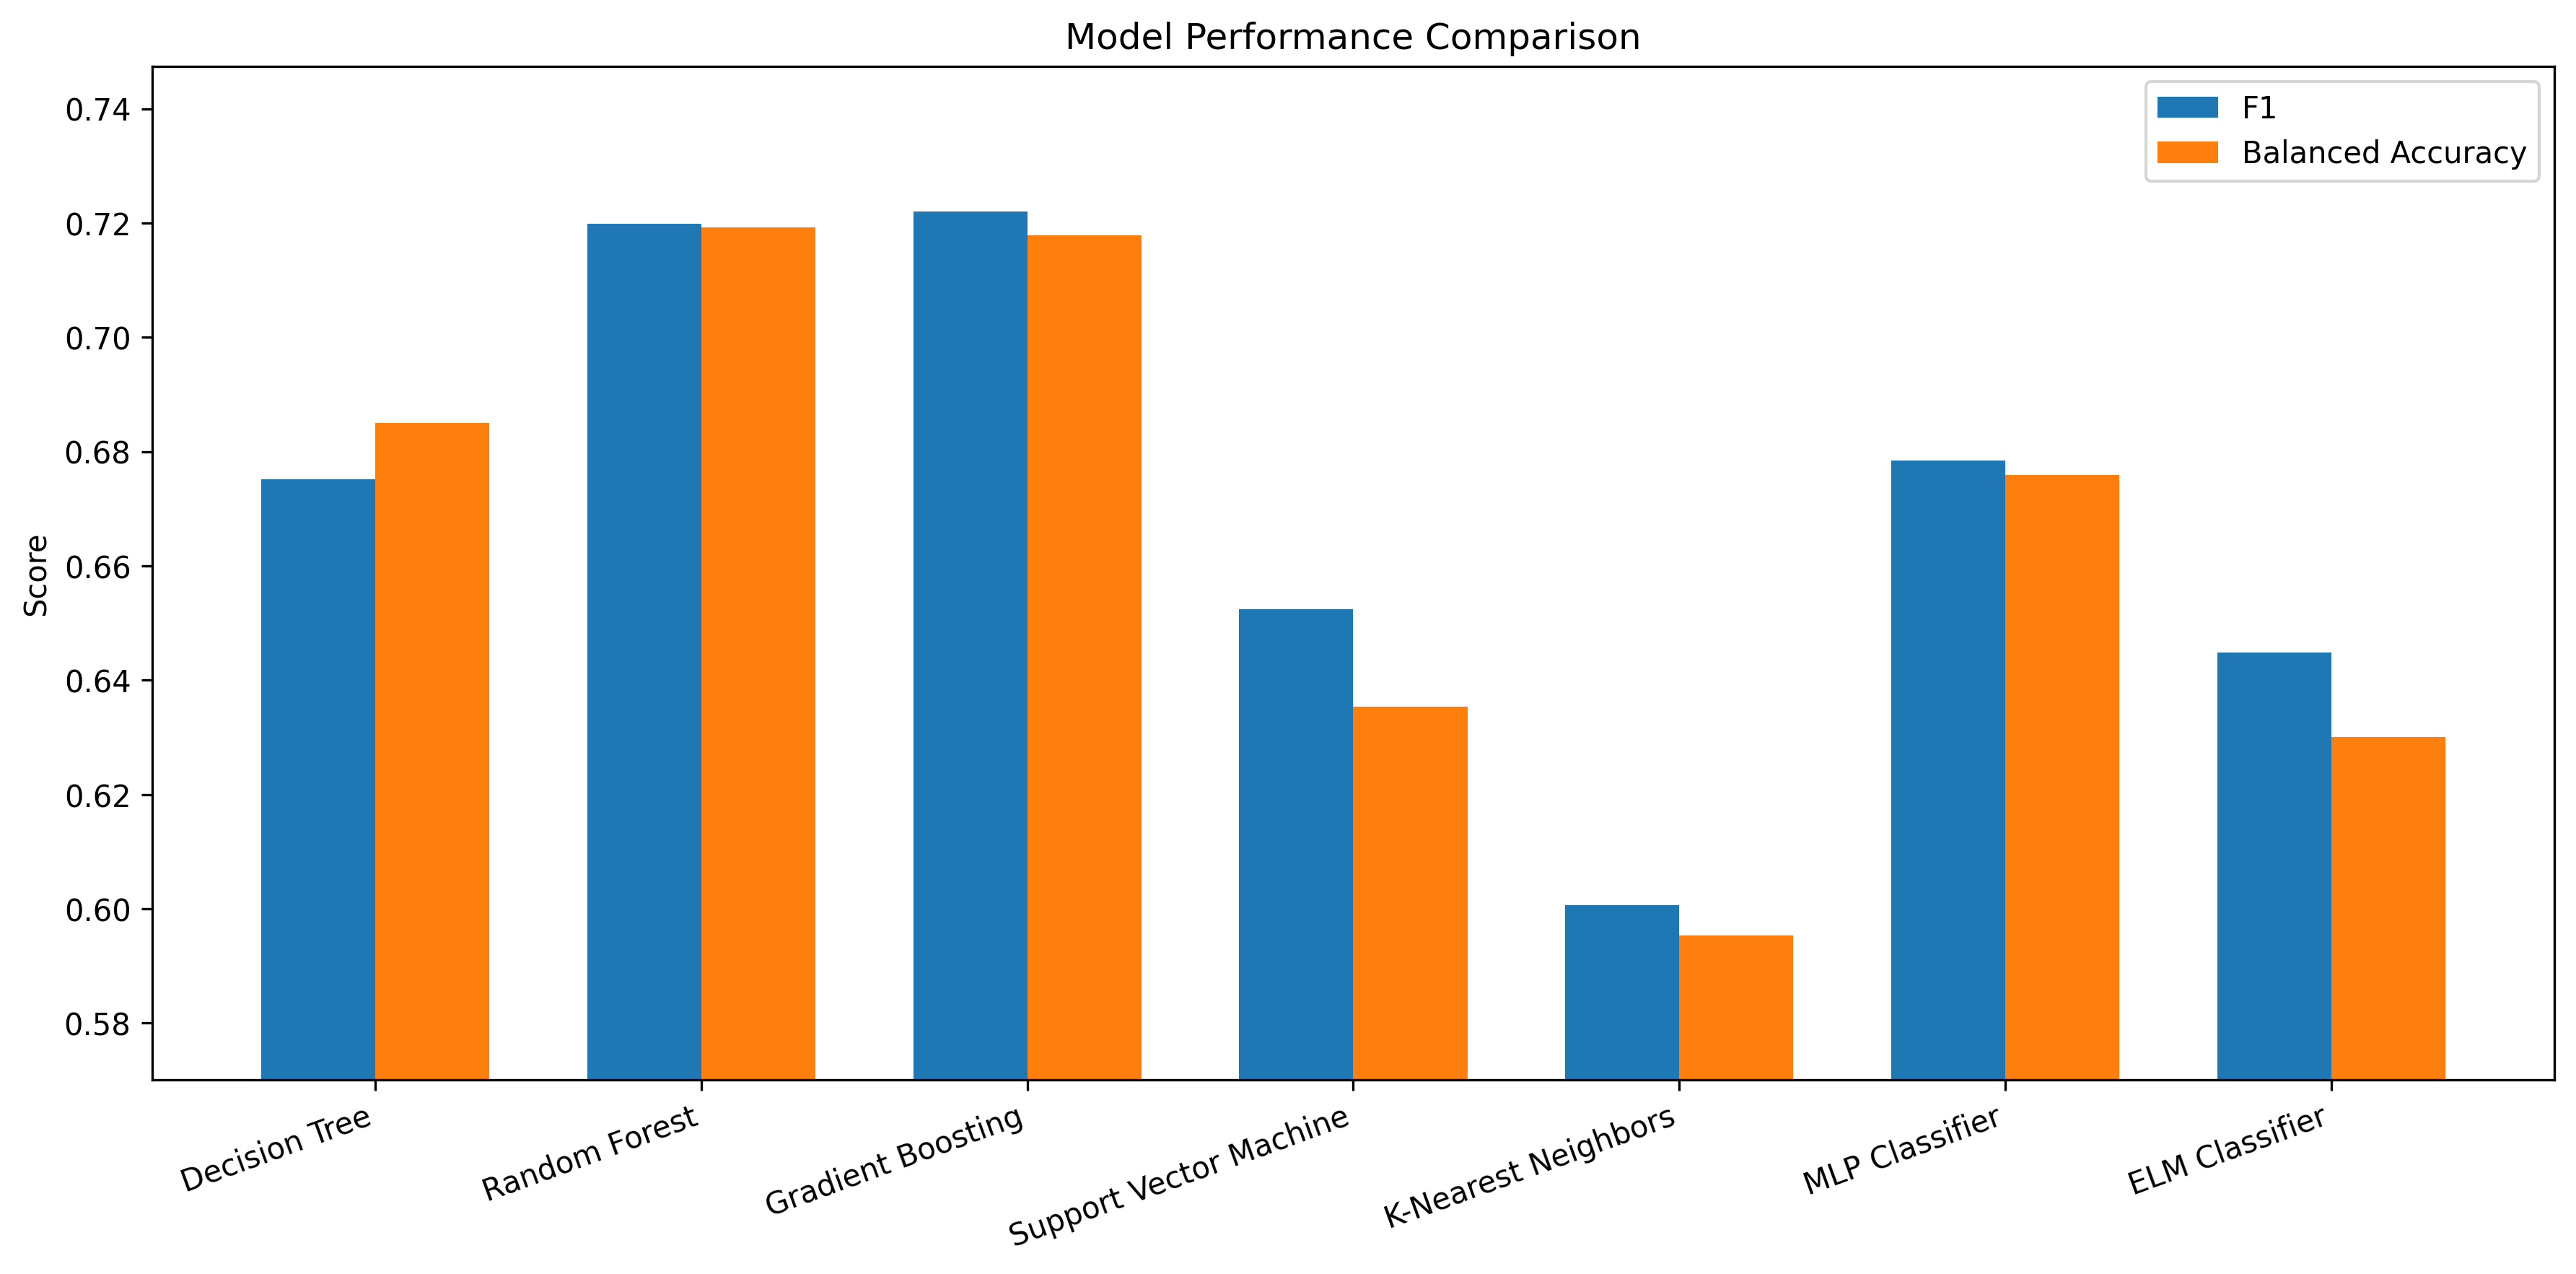
\includegraphics[width=\textwidth]{code/plots/model_performance_py.png}
	\caption{Test-set performance comparison of traditional predictive models using Macro F1 and Balanced Accuracy.}
\end{figure}

\begin{multicols}{2}

\subsection{Traditional Predictive Models}
Various traditional model architectures are implemented. The evaluated models are Random Forest, Decision Tree, Support Vector Machine, Gradient Boosting, K-Nearest Neighbors, Extreme Learning Machine, and Multi-layer Perceptron. The performance of each model is measured using plain accuracy, balanced accuracy, and F1 score. The accuracy of a model can be calculated as
\[
	\frac{\text{True Positive} + \text{True Negative}}{\text{Total Prediction}}.
\]
It is an intuitive measure of how correct the model predictions are, but falls short when the given dataset is imbalanced. To mitigate this issue, the balanced accuracy is preferred:
\[
	\frac{\text{Sensitivity} + \text{Specificity}}{2}.
\]
In addition, the F1 score is also utilized, calculated as the harmonic mean of precision and recall:
\[
	\frac{2 \times \text{Precision} \times \text{Recall}}{\text{Precision} + \text{Recall}}.
\]
As shown in Fig. 1, the model performance plot summarizes the comparative results across all evaluated traditional predictive models. We can see that ensemble methods remain the top performers, with Gradient Boosting and Random Forest achieving the highest F1 scores of 0.722 and 0.720, respectively. Support Vector Machine and Extreme Learning Machine also show competitive performance, while K-Nearest Neighbors has the lowest F1 score among the traditional models at 0.601. These results are consistent with existing literature that highlights the effectiveness of ensemble methods in classification tasks, particularly in educational contexts where complex interactions between features are common.

\subsection{Large Language Models}
\begin{figure}[H]
	\centering
	\begin{minipage}{0.5\textwidth}
		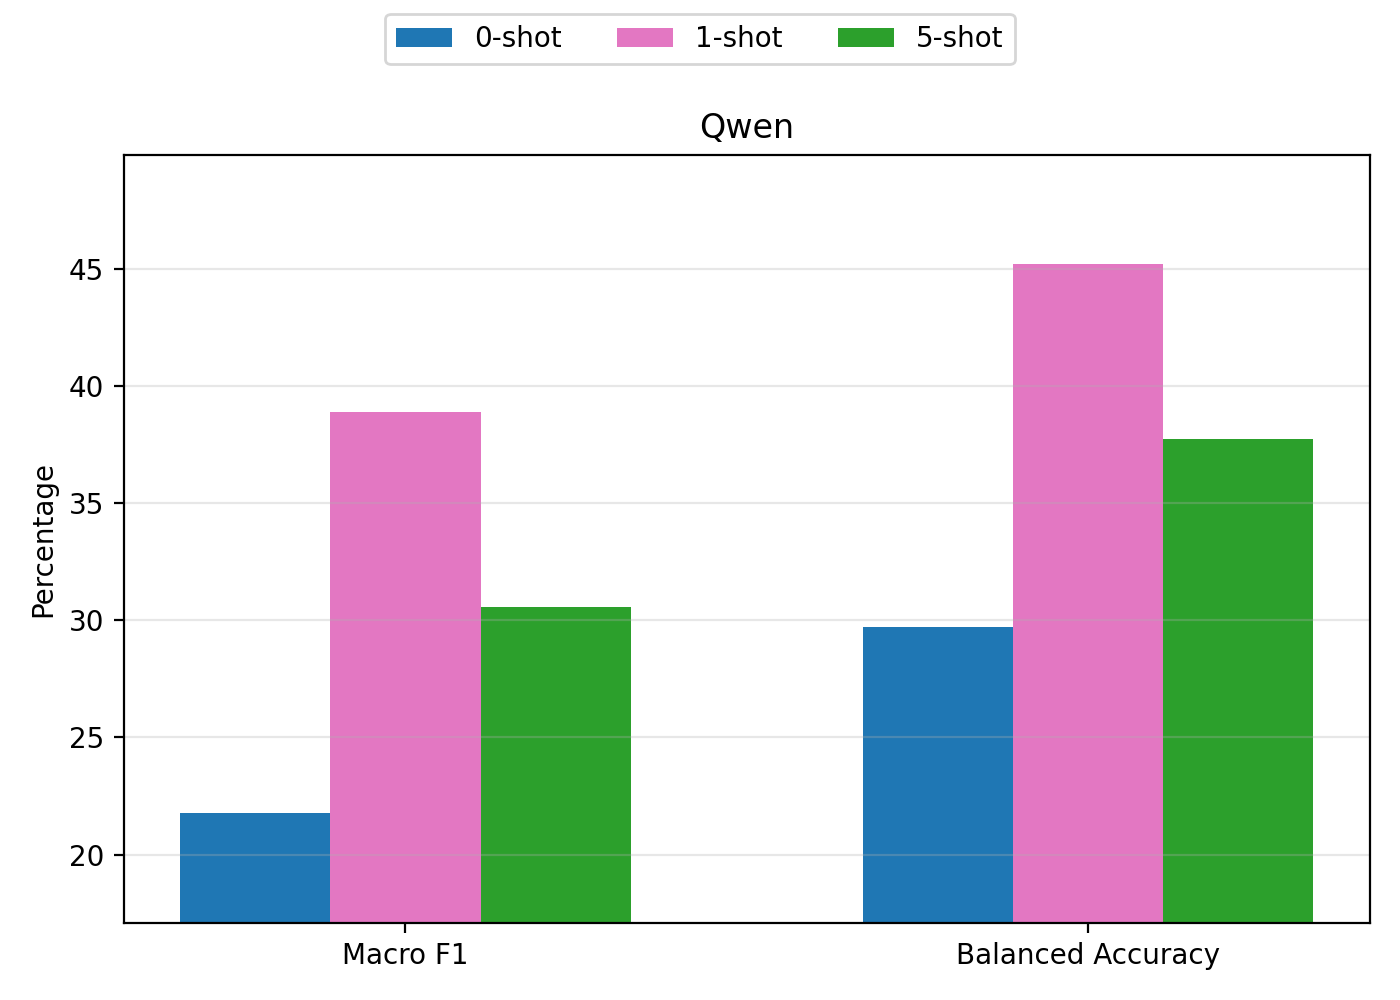
\includegraphics[width=\textwidth]{code/plots/qwen_metric_technique_comparison.png}
	\end{minipage}
	\begin{minipage}{0.5\textwidth}
		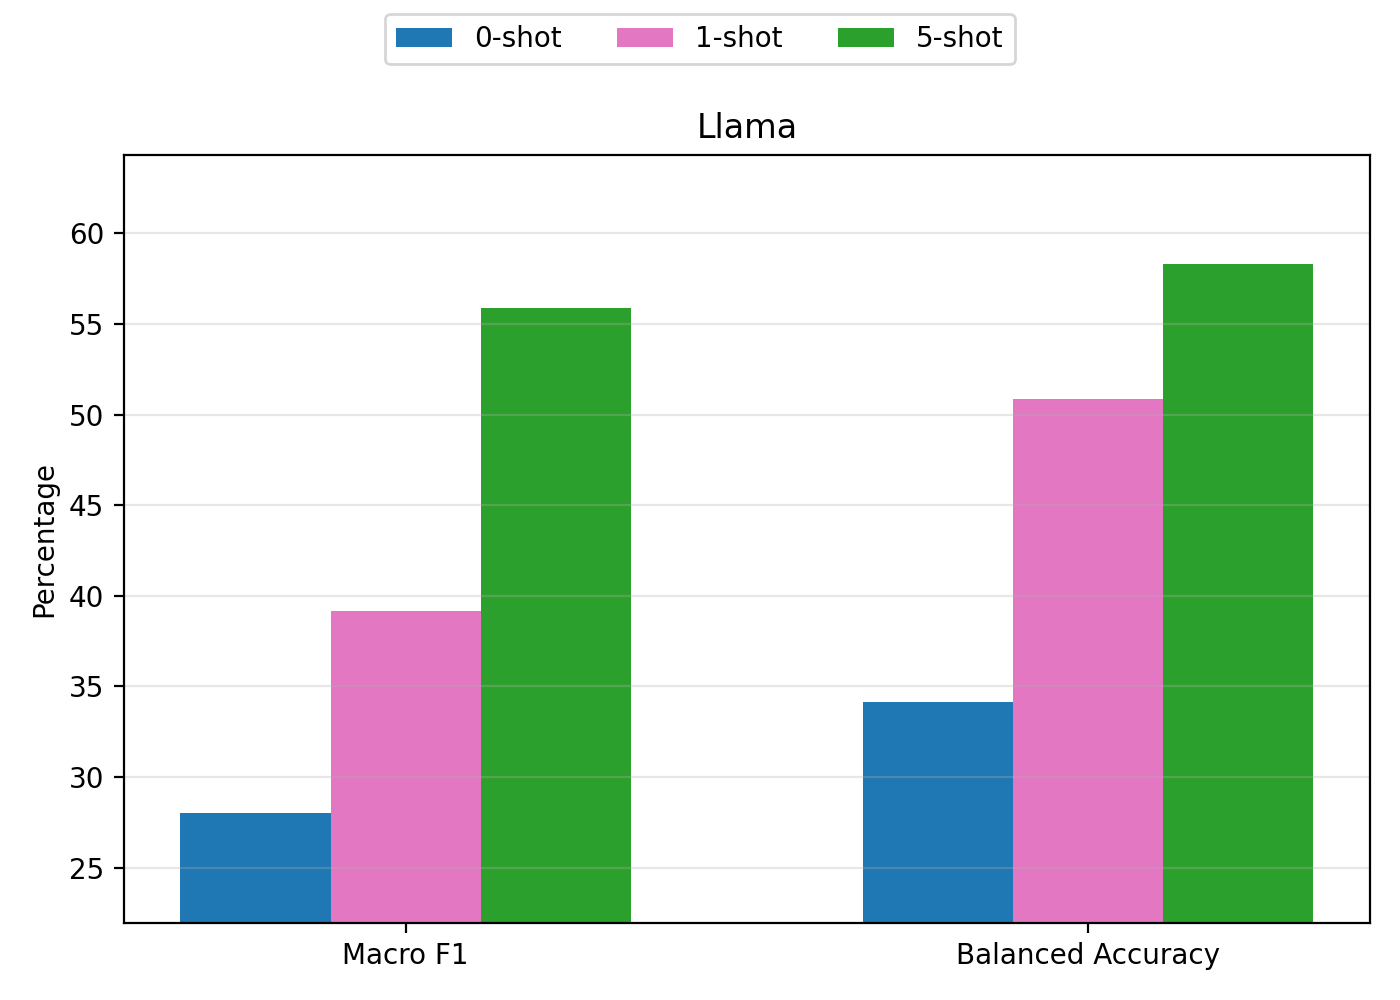
\includegraphics[width=\textwidth]{code/plots/llama_metric_technique_comparison.png}
	\end{minipage}
	\caption{Prompting-technique comparison for Qwen2.5-3B (left) and Meta-Llama3-9B (right), using Macro F1 and Balanced Accuracy.}
\end{figure}
We use a modified metric for LLMs---Macro F1. This metric effectively treats each class in a model equally important by taking the mean of the F1 scores of each class. This is particularly useful in our case, where the dataset is imbalanced, and we want to ensure that the model's performance on the minority class (e.g., at-risk students) is not overshadowed by its performance on the majority class (e.g., passing students). As shown in Fig. 1, the best performing LLM configuration is Qwen-2.5-3B with 5-shot prompting, which achieves a Macro F1 score of 0.45 and a balanced accuracy of 0.377, a performance no better than random guessing. The other LLM configurations perform even worse, with Macro F1 scores ranging from 0.218 to 0.392 and balanced accuracies between 0.297 and 0.562. 

Even the best performing LLM configuration (Qwen-2.5-3B with 5-shot prompting) achieves a Macro F1 score of only 0.45, which is significantly lower than the lowest scoring traditional model (KNN with an F1 score of 0.85). This suggests that the bottleneck is not model capacity — LLaMA-3-8B has 8 billion parameters compared to KNN's zero learned parameters — but rather the fundamental mismatch between LLM pretraining distribution (natural language) and the input modality (serialized numerical feature vectors).

This gap also contextualizes the practical implications for HEIs: at current scales, deploying general-purpose LLMs for student outcome classification without fine-tuning would produce predictions no better than a majority-class baseline, rendering them unsuitable for early-warning systems where per-class sensitivity is critical.
\section{Discussion}
\subsection{Interpretation}
The results highlight the strong performance of traditional machine learning models, particularly Gradient Boosting. In particular, Gradient Boosting predicts students' final results with a balanced accuracy of 0.718. This suggests that ensemble methods are effective at capturing the complex relationships between features in educational data, which often include a mix of demographic, behavioral, and academic indicators. The superior performance of Gradient Boosting may be attributed to its ability to sequentially correct errors made by previous models, thus enhancing overall predictive accuracy. Random Forest also performs well, closely following Gradient Boosting, which is consistent with its reputation for robustness and effectiveness in classification tasks. In contrast, simpler models like K-Nearest Neighbors show weaker performance, likely due to their sensitivity to feature scaling and inability to capture complex interactions between features.

On the other hand, LLMs show consistently weaker performance, with balanced accuracy ranging from 0.297 to 0.562 and Macro F1 ranging from 0.218 to 0.481. One contributing factor is that LLMs may fall back on default heuristics (most commonly predicting ``Fail'' or ``Pass'') when the input is a serialized feature vector rather than natural language. In our experiments, one-shot prompting yields the best balanced accuracy for both models, while five-shot prompting improves Macro F1 for LLaMA.

From a pedagogical standpoint, our study serves as a rudimentary framework for implementing an early-warning system for students. This supports the role of traditional machine learning models for this purpose and illustrates the limitations of general-purpose LLMs in structured classification problems.

\subsection{Threats to Validity}
Both approaches rely on OULAD, which lacks access to external factors that may affect students' academic performance. This includes, but is not limited to, student mental health and sudden emergencies, which may act as black swan events that reduce predictive accuracy.

There is a risk of models overfitting to historical cohorts, which may reinforce biases that do not generalize to more recent educational settings. Furthermore, students who are aware that their activities are monitored may exhibit different study patterns than those who are not, which can change the models' prediction accuracy.
\section{Conclusion}
This study presented a comparative analysis of traditional machine learning models and Large Language Models for predicting students' final outcomes based on their footprint in an online learning system and engagement patterns. The results show substantially better performance for traditional models than for general-purpose LLMs, reinforcing the effectiveness of Random Forest and Gradient Boosting as strong baselines for structured classification problems.

Our future work aims to refine the prompts fed to the LLMs for more accurate predictions, as well as evaluate larger or more capable LLMs than those used in this study. Furthermore, additional socio-economic data and more diverse datasets across disciplines would aid our analysis of the generalizability of engagement features.
\end{multicols}


%
% ---- Bibliography ----
%
% BibTeX users should specify bibliography style 'splncs04'.
% References will then be sorted and formatted in the correct style.

\printbibliography
\end{document}